
%(BEGIN_QUESTION)
% Copyright 2011, Tony R. Kuphaldt, released under the Creative Commons Attribution License (v 1.0)
% This means you may do almost anything with this work of mine, so long as you give me proper credit

This water level control system (for a municipal water supply operation) is supposed to maintain constant water level in the filter and in the clearwell.  Unfortunately, it has a problem.  Operators call you urgently to determine why the clearwell is completely empty:

$$\includegraphics[width=15.5cm]{i02326x01.eps}$$

Your first step is to ask the operator if they have actually inspected the clearwell to verify that it is empty.  They have, and it is.  They also point to the display for level controller LIC-30 and show you that it reads 0\% level.

Identify the likelihood of each specified fault for this water filtration system.  Consider each fault one at a time (i.e. no coincidental faults), determining whether or not each fault could independently account for {\it all} measurements and symptoms in this system.

% No blank lines allowed between lines of an \halign structure!
% I use comments (%) instead, so that TeX doesn't choke.

$$\vbox{\offinterlineskip
\halign{\strut
\vrule \quad\hfil # \ \hfil & 
\vrule \quad\hfil # \ \hfil & 
\vrule \quad\hfil # \ \hfil \vrule \cr
\noalign{\hrule}
%
% First row
{\bf Fault} & {\bf Possible} & {\bf Impossible} \cr
%
\noalign{\hrule}
%
% Another row
Transmitter FT-21 failed with low output &  &  \cr
%
\noalign{\hrule}
%
% Another row
Transmitter FT-21 failed with high output &  &  \cr
%
\noalign{\hrule}
%
% Another row
Transmitter LT-25 failed with low output &  &  \cr
%
\noalign{\hrule}
%
% Another row
Transmitter LT-25 failed with high output &  &  \cr
%
\noalign{\hrule}
%
% Another row
Transmitter FT-28 failed with low output &  &  \cr
%
\noalign{\hrule}
%
% Another row
Transmitter FT-28 failed with high output &  &  \cr
%
\noalign{\hrule}
%
% Another row
Transmitter LT-30 failed with low output &  &  \cr
%
\noalign{\hrule}
%
% Another row
Transmitter LT-30 failed with high output &  &  \cr
%
\noalign{\hrule}
%
% Another row
Effluent pump turned off &  &  \cr
%
\noalign{\hrule}
} % End of \halign 
}$$ % End of \vbox

Finally, identify the {\it next} diagnostic test or measurement you would make on this system.  Explain how the result(s) of this next test or measurement help further identify the location and/or nature of the fault.

\vskip 20pt \vbox{\hrule \hbox{\strut \vrule{} {\bf Suggestions for Socratic discussion} \vrule} \hrule}

\begin{itemize}
\item{} A useful problem-solving strategy for determining necessary controller actions in a cascade control system is to replace the ISA-standard ``bubble'' symbols for controllers with triangular opamp symbols, complete with ``+'' and ``$-$'' symbols at the inputs.  One input of each ``opamp'' controller will be the PV, while the other input of each ``opamp'' controller will be the SP.  The inverting and noninverting inputs standard to all operational amplifiers helps remind you that the PV and SP inputs of a loop controller always have opposite effects on the output signal.
\item{} A valuable principle to apply in a diagnostic scenario such as this is {\it correspondence}: identifying which field variables correspond with their respective controller faceplate displays, and which do not.  Apply this comparative test to the scenario described, and use it to explain why the technician's proposed test was probably not the best first step.
\end{itemize}

\underbar{file i02326}
%(END_QUESTION)





%(BEGIN_ANSWER)

\noindent
{\bf Partial answer:}

% No blank lines allowed between lines of an \halign structure!
% I use comments (%) instead, so that TeX doesn't choke.

$$\vbox{\offinterlineskip
\halign{\strut
\vrule \quad\hfil # \ \hfil & 
\vrule \quad\hfil # \ \hfil & 
\vrule \quad\hfil # \ \hfil \vrule \cr
\noalign{\hrule}
%
% First row
{\bf Fault} & {\bf Possible} & {\bf Impossible} \cr
%
\noalign{\hrule}
%
% Another row
Transmitter FT-21 failed with low output &  &  \cr
%
\noalign{\hrule}
%
% Another row
Transmitter FT-21 failed with high output &  &  \cr
%
\noalign{\hrule}
%
% Another row
Transmitter LT-25 failed with low output &  & $\surd$ \cr
%
\noalign{\hrule}
%
% Another row
Transmitter LT-25 failed with high output &  &  \cr
%
\noalign{\hrule}
%
% Another row
Transmitter FT-28 failed with low output &  &  \cr
%
\noalign{\hrule}
%
% Another row
Transmitter FT-28 failed with high output & $\surd$ &  \cr
%
\noalign{\hrule}
%
% Another row
Transmitter LT-30 failed with low output &  &  \cr
%
\noalign{\hrule}
%
% Another row
Transmitter LT-30 failed with high output &  &  \cr
%
\noalign{\hrule}
%
% Another row
Effluent pump turned off &  &  \cr
%
\noalign{\hrule}
} % End of \halign 
}$$ % End of \vbox

%(END_ANSWER)





%(BEGIN_NOTES)

Since we are told the clearwell is actually empty, we may conclude the problem is not with LT-30 because that's telling us the same thing.

% No blank lines allowed between lines of an \halign structure!
% I use comments (%) instead, so that TeX doesn't choke.

$$\vbox{\offinterlineskip
\halign{\strut
\vrule \quad\hfil # \ \hfil & 
\vrule \quad\hfil # \ \hfil & 
\vrule \quad\hfil # \ \hfil \vrule \cr
\noalign{\hrule}
%
% First row
{\bf Fault} & {\bf Possible} & {\bf Impossible} \cr
%
\noalign{\hrule}
%
% Another row
Transmitter FT-21 failed with low output &  & $\surd$ \cr
%
\noalign{\hrule}
%
% Another row
Transmitter FT-21 failed with high output & $\surd$ &  \cr
%
\noalign{\hrule}
%
% Another row
Transmitter LT-25 failed with low output &  & $\surd$ \cr
%
\noalign{\hrule}
%
% Another row
Transmitter LT-25 failed with high output & $\surd$ &  \cr
%
\noalign{\hrule}
%
% Another row
Transmitter FT-28 failed with low output &  & $\surd$ \cr
%
\noalign{\hrule}
%
% Another row
Transmitter FT-28 failed with high output & $\surd$ &  \cr
%
\noalign{\hrule}
%
% Another row
Transmitter LT-30 failed with low output &  & $\surd$ \cr
%
\noalign{\hrule}
%
% Another row
Transmitter LT-30 failed with high output &  & $\surd$ \cr
%
\noalign{\hrule}
%
% Another row
Effluent pump turned off &  & $\surd$ \cr
%
\noalign{\hrule}
} % End of \halign 
}$$ % End of \vbox










\filbreak \vskip 20pt \vbox{\hrule \hbox{\strut \vrule{} {\bf Virtual Troubleshooting} \vrule} \hrule}

\noindent
{\bf Predicting the effect of a given fault:} present each of the following faults to the students, one at a time, having them comment on all the effects each fault would produce.

\begin{itemize}
\item{} Power fails to FV-21
\item{} Power fails to FV-28
\item{} FT-21 transmitter fails with low signal
\item{} FT-21 transmitter fails with high signal
\item{} LT-25 transmitter fails with low signal
\item{} LT-25 transmitter fails with high signal
\item{} FT-28 transmitter fails with low signal
\item{} FT-28 transmitter fails with high signal
\item{} LT-30 transmitter fails with low signal
\item{} LT-30 transmitter fails with high signal
\item{} Influent pump shuts off
\item{} Effluent pump shuts off
\end{itemize}


\vskip 10pt


\noindent
{\bf Identifying possible/impossible faults:} present symptoms to the students and then have them determine whether or not a series of suggested faults could account for all the symptoms, explaining {\it why} or {\it why not} for each proposed fault:

\begin{itemize}
\item{} Symptom: {\it Clearwell is overflowing; FT-28 trend is flat-lined at a normal amount of flow}
\item{} LT-30 failed with low signal -- {\bf No}
\item{} LT-30 failed with high signal -- {\bf No}
\item{} FV-28 power failure -- {\bf Yes}
\item{} LT-25 failed with low signal -- {\bf No}
\item{} LT-25 failed with high signal -- {\bf No}
\item{} FV-21 failed fully open -- {\bf No}
\item{} FT-21 failed with low signal -- {\bf No}
\item{} FT-21 failed with high signal -- {\bf No}
\item{} FIC-28 in manual mode -- {\bf Yes}
\end{itemize}


\vskip 10pt


\noindent
{\bf Determining the utility of given diagnostic tests:} present symptoms to the students and then propose the following diagnostic tests one by one.  Students rate the value of each test, determining whether or not it would give useful information (i.e. tell us something we don't already know).  Students determine what different results for each test would indicate about the fault, if anything:

\begin{itemize}
\item{} Symptom: {\it Clearwell level is below setpoint (visual inspection)}
\item{} Check LT-30 (level) trend graph -- {\bf Yes}
\item{} Inspect FV-28 stem position -- {\bf No} (not until we have reason to believe the control valve may not be responding properly to FIC-28's output)
\item{} Check LIC-30 output trend graph -- {\bf Yes}
\item{} Check FIC-28 (flow) trend graph -- {\bf No} (not until we have checked to see that LIC-30 is taking the correct action)
\item{} Check LT-25 (level) trend graph -- {\bf Yes}
\item{} Check effluent pump status -- {\bf No}
\item{} Check for shut valves on influent line -- {\bf No} (not until insufficient flow has been revealed by other tests)
\end{itemize}


\vskip 10pt

\filbreak


\noindent
{\bf Diagnosing a fault based on given symptoms:} imagine the ??? fails ??? in this system (don't reveal the fault to students!).  Present the operator's observation(s) to the students, have them consider possible faults and diagnostic strategies, and then tell them the results of tests they propose based on the following symptoms, until they have properly identified the nature and location of the fault:

\begin{itemize}
\item{} {\it }
\item{} 
\item{} 
\end{itemize}

%INDEX% Basics, control loop troubleshooting: determining cause of control problem
%INDEX% Control, strategies: cascade
%INDEX% Process: water filter flow/level control

%(END_NOTES)


